%!TEX root = ../../main.tex

\chapter{Clickable Elements}
All elements that are clickable must have a safety-distance to other elements. This will ensure that the user does not accidentally press the wrong thing and ultimately does something wrong. This safety distance may be achieved using several different methods. Please refer to the following sections. Figure \ref{fig:correct_element_spacing} shows an example of correct item spacing while \ref{fig:incorrect_element_spacing} shows an example of incorrect item spacing.
\\\\
Elements must have a safety distance to \ldots
\begin{itemize}
	\item Other clickable elements
	\item Borders of it's container
	\item Borders of the tablet
\end{itemize}

\begin{figure}[!htbp]
    \centering

    \begin{subfigure}[t]{0.4\textwidth}
    	\centering
        
\includegraphics[scale=0.1]{correct_element_spacing}
        \caption{Correct item spacing}
        \label{fig:correct_element_spacing}
    \end{subfigure}
    \hspace{5em} 
    \begin{subfigure}[t]{0.4\textwidth}
    	\centering
        
\includegraphics[scale=0.1]{incorrect_element_spacing}
        \caption{Incorrect item spacing}
        \label{fig:incorrect_element_spacing}
    \end{subfigure}
    
    \caption{Examples of correct and incorrect element spacing}
    \label{fig:element_spacing_examples}
\end{figure}

\section{Element Margin}
Elements may be spaced apart from each other using margin on the individual elements. The distance between the elements should be consistent throughout all activities of any given application. Figure \ref{fig:element_margin_example} shows an example of the margin for a given element.. 

\begin{figure}[h]
	\centering
	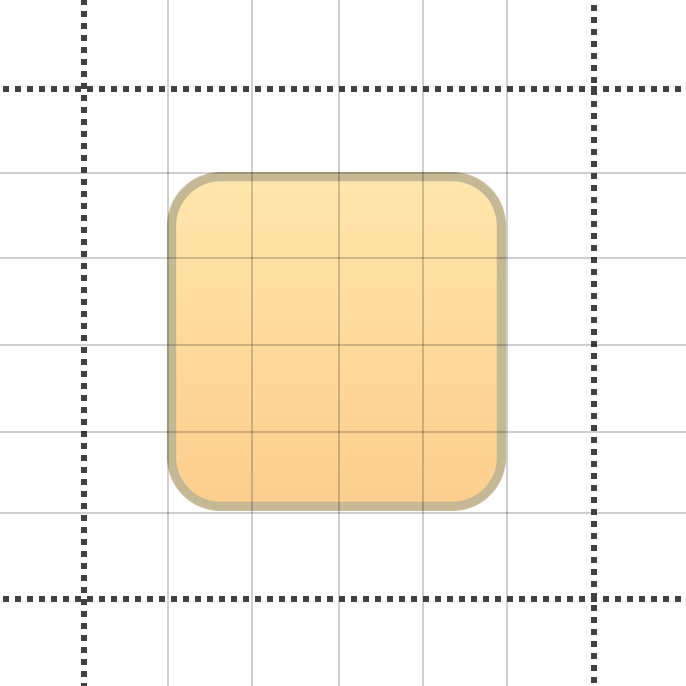
\includegraphics[width=0.25\textwidth]{element_margin_example}
	\caption{Example of element margin}
	\label{fig:element_margin_example}
\end{figure}

\begin{note}
	If margin is used inside a container each element with margin will also be a certain distance from the borders of that specific container. If, for instance, an element has a margin of $10$, then this element would be a distance of $10$ from the borders of the container. This means that there \textit{might} not be need for any padding on the given container.
\end{note}

\subsection{Consistent Margin}
Elements of the same type appearing in the same context must have the same distance to other elements. However, if the elements appear in an order, for example a horizontal list, the first and last element may differ. For instance, the first element may have a smaller left-margin and the last element may have a smaller right-margin. Figure \ref{fig:element_margin_consistency} shows an illustration of this example.

\begin{figure}[h]
	\centering
	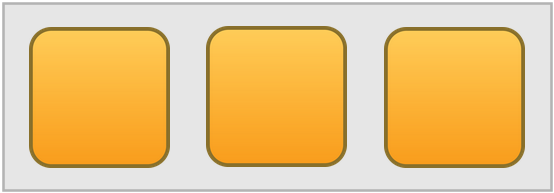
\includegraphics[width=0.45\textwidth]{element_margin_consistency}
	\caption{Example of element margin}
	\label{fig:element_margin_consistency}
\end{figure}


\section{Container Padding}
Each container should provide some padding for its content. This padding should be somewhat identical to the spacing between elements inside the container. Figure \ref{fig:container_padding_example} shows an example of a container with padding. 

\begin{figure}[h]
	\centering
	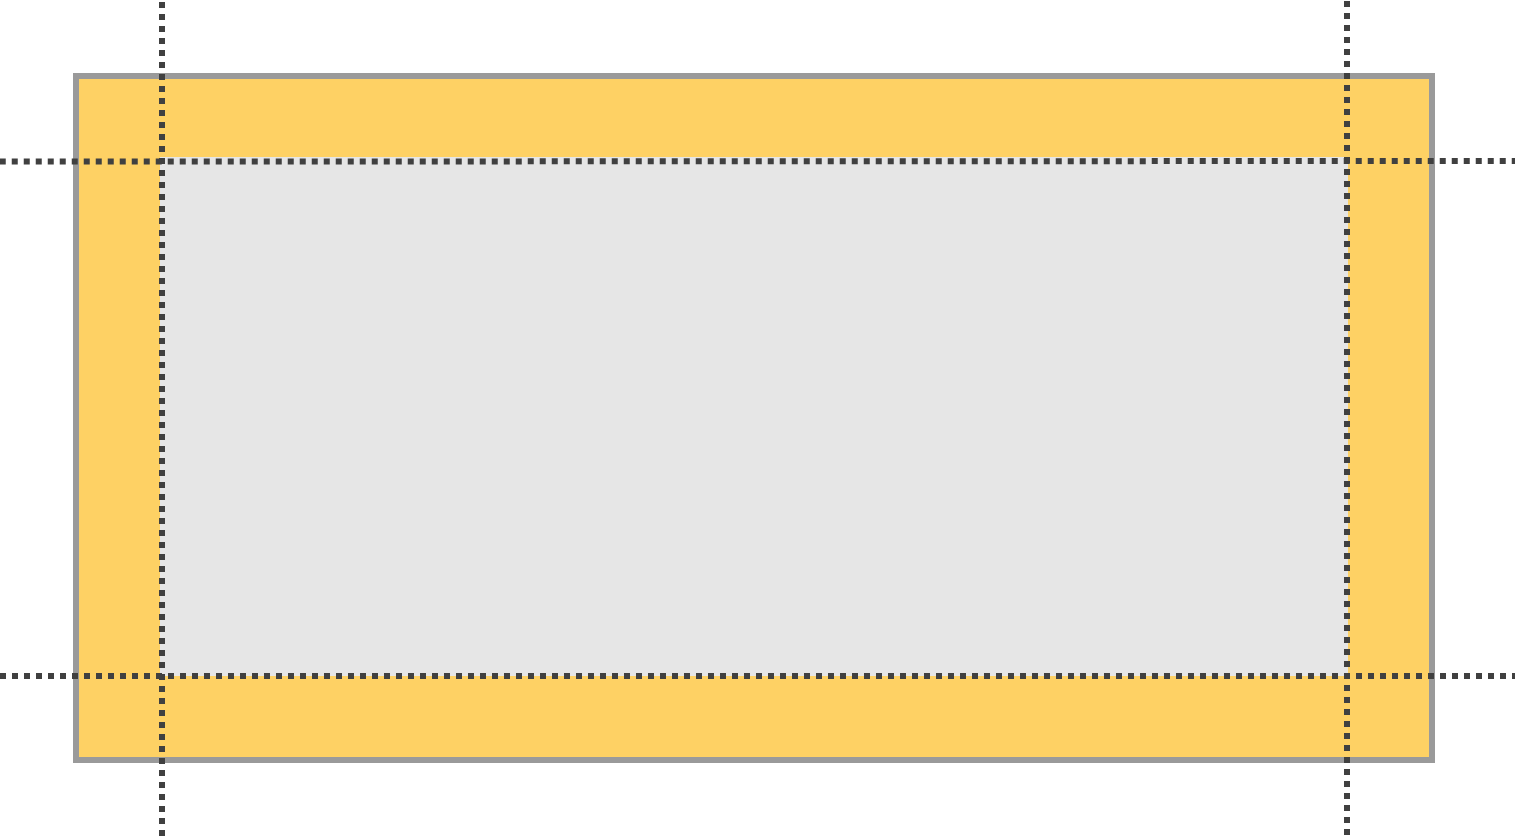
\includegraphics[width=0.65\textwidth]{container_padding_example}
	\caption{Example of a container with padding}
	\label{fig:container_padding_example}
\end{figure}

\begin{note}
	Whenever the content of the container can be scrolled through (for example a \texttt{GridView}) a property called \texttt{clipToPadding} must be set to \texttt{false}. Please refer to the \href{http://developer.android.com/reference/android/view/ViewGroup.html#attr_android:clipToPadding}{Android documentation} for additional information.
\end{note}\todo{The effect of this could be explained more clearly using a figure}
